%%% for platex
\documentclass[dvipdfmx,a4paper,12pt]{jbook}
%%% for lualatex
%\documentclass[a4paper,12pt]{ltjbook}

\usepackage{bachelor}
%%%%%%%%%%%%%%%%%%%%%%%%%%%%%%%%%%%%%%%%%%%%%%%%%%%%%%%%%%%%%%%%
% User-defined Macro
%%%%%%%%%%%%%%%%%%%%%%%%%%%%%%%%%%%%%%%%%%%%%%%%%%%%%%%%%%%%%%%%
\newcommand{\compress}{\itemsep0pt\parsep0pt\parskip0pt\partopsep0pt}
% \newcommand{\compress}{\itemsep1pt plus1pt\parsep0pt\parskip0pt}
% \newcommand{\code}[1]{\lstinline[basicstyle=\ttfamily]{#1}}
\newcommand{\gringo}{\textit{gringo}}
\newcommand{\clasp}{\textit{clasp}}
\newcommand{\clingo}{\textit{clingo}}
\newcommand{\teaspoon}{\textit{teaspoon}}
\newcommand{\sat}{\textsf{SAT}}
\newcommand{\unsat}{\textsf{UNSAT}}
% \newcommand{\web}[2]{\href{#1}{#2\ \raisebox{-0.15ex}{\beamergotobutton{Web}}}}
% \newcommand{\doi}[2]{\href{#1}{#2\ \raisebox{-0.15ex}{\beamergotobutton{DOI}}}}
% \newcommand{\weblink}[1]{\web{#1}{#1}}
% \newcommand{\imp}{\mathrel{\Rightarrow}}
% \newcommand{\Iff}{\mathrel{\Leftrightarrow}}
% \newcommand{\mybox}[1]{\fbox{\rule[.2cm]{0cm}{0cm}\mbox{${#1}$}}}
% \newcommand{\mycbox}[2]{\tikz[baseline]\node[fill=#1!10,anchor=base,rounded corners=2pt] () {#2};}
% \newcommand{\naf}[1]{\ensuremath{{\sim\!\!{#1}}}}
% \newcommand{\head}[1]{\ensuremath{\mathit{head}(#1)}}
% \newcommand{\body}[1]{\ensuremath{\mathit{body}(#1)}}
% \newcommand{\atom}[1]{\ensuremath{\mathit{atom}(#1)}}
% \newcommand{\poslits}[1]{\ensuremath{{#1}^+}}
% \newcommand{\neglits}[1]{\ensuremath{{#1}^-}}
% \newcommand{\pbody}[1]{\poslits{\body{#1}}}
% \newcommand{\nbody}[1]{\neglits{\body{#1}}}
% \newcommand{\Cn}[1]{\ensuremath{\mathit{Cn}(#1)}}
% \newcommand{\reduct}[2]{\ensuremath{#1^{#2}}}
% \newcommand{\OK}{\mbox{\textcolor{green}{\Pisymbol{pzd}{52}}}}
% \newcommand{\KO}{\mbox{\textcolor{red}{\Pisymbol{pzd}{56}}}}
% \newcommand{\code}[1]{\lstinline[basicstyle=\ttfamily]{#1}}
% \newcommand{\lw}[1]{\smash{\lower2.ex\hbox{#1}}}
\newcommand{\llw}[1]{\smash{\lower3.ex\hbox{#1}}}

\newenvironment{tableC}{%
  \scriptsize
  \renewcommand{\arraystretch}{0.9}
  \tabcolsep = 0.6mm
  % \begin{tabular}[t]{p{6mm}|rlr|rlr|rlr|rlr|rlr}\hline
  %   \multicolumn{1}{l|}{\llw{問題   }} &
  \begin{tabular}[t]{l|rlr|rlr|rlr|rlr|rlr}\hline
    \multicolumn{1}{l|}{\llw{問題}} &
    \multicolumn{3}{c|}{UD1} &
    \multicolumn{3}{c|}{UD2} &
    \multicolumn{3}{c|}{UD3} &
    \multicolumn{3}{c|}{UD4} &
    \multicolumn{3}{c}{UD5} \\
    & 
    \multicolumn{1}{c}{既知の} & & \multicolumn{1}{c|}{ASP} & 
    \multicolumn{1}{c}{既知の} & & \multicolumn{1}{c|}{ASP} & 
    \multicolumn{1}{c}{既知の} & & \multicolumn{1}{c|}{ASP} & 
    \multicolumn{1}{c}{既知の} & & \multicolumn{1}{c|}{ASP} & 
    \multicolumn{1}{c}{既知の} & & \multicolumn{1}{c}{ASP} \\
    & 
    ベスト & &  & 
    ベスト & &  & 
    ベスト & &  & 
    ベスト & &  & 
    ベスト & &  \\
    \hline
  }{%
    \hline
  \end{tabular}
}
 % 自分用のマクロ

%%%%%%%%%%%%%%%%%%%%%%%%%%%%%%%%%%%%%%%%%%%%%%%%%%%%%%%%%%
% タイトル
%%%%%%%%%%%%%%%%%%%%%%%%%%%%%%%%%%%%%%%%%%%%%%%%%%%%%%%%%%
\school{名古屋大学情報学部}
\bookname{コンピュータ科学科卒業論文}
\title{解集合プログラミングを用いた\\組合せ遷移問題の解法に関する考察}
\date{2021年2月}
\author{山田 悠也}

%%%%%%%%%%%%%%%%%%%%%%%%%%%%%%%%%%%%%%%%%%%%%%%%%%%%%%%%%% 
% 本体
%%%%%%%%%%%%%%%%%%%%%%%%%%%%%%%%%%%%%%%%%%%%%%%%%%%%%%%%%% 
\begin{document}
\maketitle

%%%%%%%%%%%%%%%%%%%%%%%%%%%%%%%%%%%%%%%%%%%%%%%%%%%%%%%%%% 
\chapter*{概要}
\pagenumbering{roman}
%%%%%%%%%%%%%%%%%%%%%%%%%%%%%%%%%%%%%%%%%%%%%%%%%%%%%%%%%% 

本論文では,解集合プログラミングを用いた組合せ遷移問題の解法について述べる.
組合せ遷移問題とは,ある組合せ問題とその2つの実行可能解が与えられたとき,
一方の実行可能解から他方の実行可能解へ,
遷移制約を満たしつつ到達できるかを判定する問題である.

$k$彩色遷移問題は組合せ遷移問題の一つであり,
色数$k$のグラフ点彩色問題と二つの彩色が与えられたとき,
一方の彩色から他方の彩色へ,各遷移過程において色が変化する頂点はただ一つ
という遷移制約を満たしつつ,到達できるかを判定する問題である.
一般に,$k \ge 4$において PSPACE 完全であることが知られている.

解集合プログラミング(ASP)は,論理プログラムから派生したプログラミングパラダイムである.
ASP 言語は一階論理に基づいた知識表現言語の一種である.
論理プログラムはルールの有限集合である.
ASP システムは解集合を計算するシステムである.

本論文では,解集合プログラミング(ASP)を用いた$k$彩色遷移問題の解法について述べる.
本研究では問題の入力に遷移回数$t$を加え,「遷移回数$t$での経路の存在」を解く.
まず,$k$彩色遷移問題を解く3種類の ASP 符号化,
\code{vrc1},\code{vrc2},\code{vrc3}を提案した.
特に\code{vrc3}では基礎化後のルール数を少なく抑えているため,
大規模な問題に対する有効性が期待できる.

提案した符号化を評価するにあたり,
独自に生成した90問のベンチマークを使用し評価実験を行った.
その結果,すべての符号化で90問中11問で到達可能であることを判定できた.
さらに,\textsf{vrc3}符号化は,多くの問題で判定に要した CPU 時間が短く,
その優位性が確認できた.

%%% Local Variables:
%%% mode: japanese-latex
%%% TeX-master: "paper"
%%% End:    % 概要

\tableofcontents    % 目次
%\listoffigures      % 図の目次
%\listoftables       % 表の目次
%\lstlistoflistings  % コードの目次

% ここから「本文」
%%%%%%%%%%%%%%%%%%%%%%%%%%%%%%%%%%%%%%%%%%%%%%%%%%%%%%%%%% 
\chapter{序論}
\pagenumbering{arabic}
%%%%%%%%%%%%%%%%%%%%%%%%%%%%%%%%%%%%%%%%%%%%%%%%%%%%%%%%%% 

\textbf{ハミルトン閉路問題 (Hamiltonian Cycle Problem)} は,
与えられたグラフの全頂点をちょうど一度ずつ通る閉路が存在するかどうかを
判定する問題である.
\textbf{ハミルトン路問題 (Hamiltonian Path Problem)} は,
ハミルトン閉路問題から始点と終点が一致するという閉路の条件を取り除いた
ものである.
ハミルトン閉路問題とハミルトン路問題は,どちらも NP 完全な問題である.
これらの問題は,重要な工学的応用が数多く存在するため,古くから盛んに研
究されている.
例えば,数理最適化の分野で有名な巡回セールスマン問題は,グラフの辺に距
離が付随しているとき,最短距離のハミルトン閉路を求める
\textbf{最短ハミルトン閉路問題}と考えることができる.
また,ごく最近では,距離の総和が所与の閾値以下(または以上)であることを
制約条件として付加した
\textbf{コスト制約付きハミルトン閉路問題}\cite{comp20:Minato}
も提案されている.
本研究では,無向グラフ上のハミルトン閉路問題およびその関連問題を対象とする.

解集合プログラミング(Answer Set Programming; ASP)は,
論理プログラミングから派生した比較的新しいプログラミングパラダイムである.
ASP言語は,一階論理に基づく知識表現言語の一種であり,
論理プログラムは ASP のルールの有限集合である.
ASP システムは論理プログラムから安定モデル意味論に基づく解集合を計算す
るシステムである.
近年,SAT技術を応用した高速 ASP システムが開発され,スケジューリング,
プランニング,システム生物学,システム検証,制約充足問題,
制約最適化問題など様々な分野への実用的応用が急速に拡大している.
ハミルトン閉路問題およびその関連問題に対して ASP を用いる利点としては,
ASP 言語の高い表現力,
充足不能コアに基づく最適化,
インクリメンタルASP解法,
組込み非閉路制約,
高速な解列挙
などが挙げられる.

本論文では,解集合プログラミング(ASP)を用いた
ハミルトン閉路問題,
最短ハミルトン閉路問題,
コスト制約付きハミルトン閉路問題
の解法について述べる.
%
ハミルトン閉路問題を解くASP符号化として,
\textsf{undirected},
\textsf{directed},
\textsf{acyclicity}
の3つを考案した.
\textsf{undirected}は,
ハミルトン閉路問題を次数制約と部分閉路禁止制約で簡潔に表現した符号化である.
\textsf{directed}は,
与えられた無向グラフの各辺$u-v$に対して,
2つの弧$u\rightarrow v$と$v\rightarrow u$を対応させることで有向グラフ
化して解く符号化である.
変換した有向グラフ上のハミルトン閉路は元の無向グラフ上のハミルトン閉路
となり,また逆も成り立つ.
\textsf{acyclicity}は,\textsf{directed}符号化をベースに,
部分閉路禁止制約を組込み非閉路制約で表現した符号化である.
\textsf{acyclicity}符号化は,他の二つと比較して,基礎化後の制約数を少
なく抑えることができるため,大規模な問題に対する有効性が期待できる.
最短ハミルトン閉路問題とコスト制約付きハミルトン閉路問題については,
考案した3つの符号化に目的関数とコスト制約をそれぞれ追加することで自然に拡張できる.

考案した符号化の有効性を評価するために,
既存のベンチマーク問題集(7種類,計516問)を用いて実行実験を行なった.
その結果,
ハミルトン閉路問題とコスト制約付きハミルトン閉路問題(解の全列挙)について,
\textsf{acyclicity}符号化が,
\textsf{undirected}と\textsf{directed}と比較して,
より多くの問題を高速に解くことに成功し,その優位性を確認できた.
また,最短ハミルトン閉路問題については,
\textsf{undirected}符号化が,他の符号化と比較して,より多くの問題で最
適値・最良値を求めることができた.

%%% Local Variables:
%%% mode: latex
%%% TeX-master: "paper"
%%% End:

\section{CAFE問題}\label{sec:background}

%-------------------------------------------------------
\begin{figure*}[t]
  \centering
  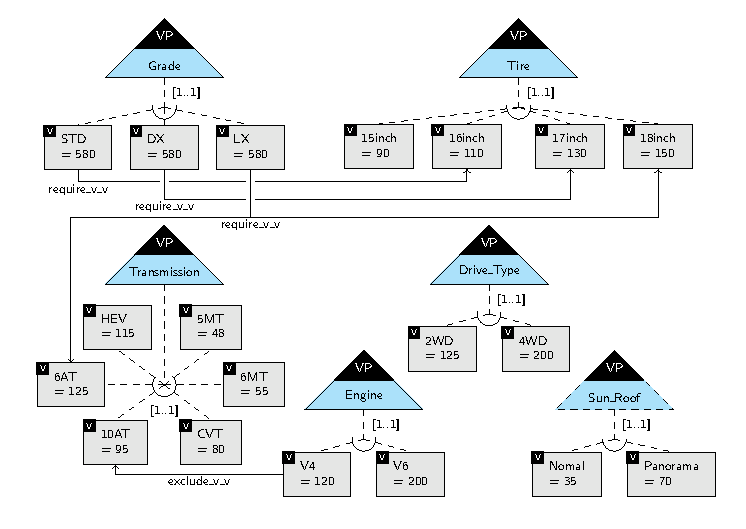
\includegraphics[width=0.8\linewidth]{images/ovm_example.eps}
  \caption{CAFE問題の例}
  \label{fig:ovm_example}
\end{figure*}
%-------------------------------------------------------

CAFE問題の入力は以下の通りである.
以降,
装備タイプをタイプ,
装備オプションをオプション
と簡単に書くことにする.
\begin{enumerate}
\item タイプの集合\label{input:vp}
\item オプションの集合\label{input:v}
\item タイプとオプションの対応関係\label{input:vp-v}
\item 各タイプで選択可能なオプション数の上下限値\label{input:ublb}
\item タイプ同士,オプション同士,および,タイプとオプション間の依存関係
  \label{input:dependency}
\item 各オプションに付加された IWR 値\label{input:iwr}
%%%
\item 求めたい装備仕様の個数\label{input:g}
\item 各装備仕様とタイプ(あるいはオプション)間の依存関係\label{input:init}
\item 各装備仕様に含まれるオプションの IWR 値の総和と燃費との対応表\label{input:fe}
\item 各装備仕様に含まれるオプションの IWR 値の総和と予想販売台数との対応表\label{input:sv}
\item CAFE 基準値\label{input:cafe}
\end{enumerate}
入力~\ref{input:iwr}の IWR は Inertial Working Rating の略で,
直観的には各オプションの重量を表す.
入力~\ref{input:g}の個数は,求めたい派生車両の数と考えるとわかりやすい.
CAFE問題は,上記の入力から,
装備および燃費に関する制約を満たしつつ,
予想販売台数を最大化する車両装備仕様を求める問題である.

CAFE問題の制約は以下の通りである.
\begin{description}
\item[範囲制約]: 各装備仕様について,各タイプで選択されるオプション数は,
  入力~\ref{input:ublb}で与えられた上下限値の範囲内でなければならない.
\item[依存制約]: 各装備仕様について,入力~\ref{input:dependency}で与
  えられた依存関係を満たさなければならない.
  依存制約には,要求制約と排他制約の2つがある.
\item[燃費制約]: 入力~\ref{input:cafe}の CAFE 基準値を$t$,
  入力~\ref{input:g}の装備仕様個数を$n$として,
  以下の CAFE 規制を満たさなければならない.
  \[
    \begin{array}{lcr}
      & & \\
      \displaystyle\frac{\sum_{i=1}^{n} FE_{i}\cdot SV_{i}}{\sum_{i=1}^{n} SV_{i}}
      &
        \geq 
      &
        t \\
      & & 
    \end{array}
  \]
  不等式の左辺は$n$個の装備仕様の\textbf{平均燃費}を表している.
  $FE_{i}$と$SV_{i}$は,装備仕様$i$の燃費と予想販売台数を表しており,
  それぞれ,入力~\ref{input:fe}と\ref{input:sv}の対応表を元に計算される.
\item[初期制約]:
  入力~\ref{input:init}で与えられた依存関係を満たさなければならない.
\end{description}

%%%%%%%%%%%%%%%%%%%%%%%%%%%%
%-------------------------------------------------------
\begin{figure}[tb]
  \centering
  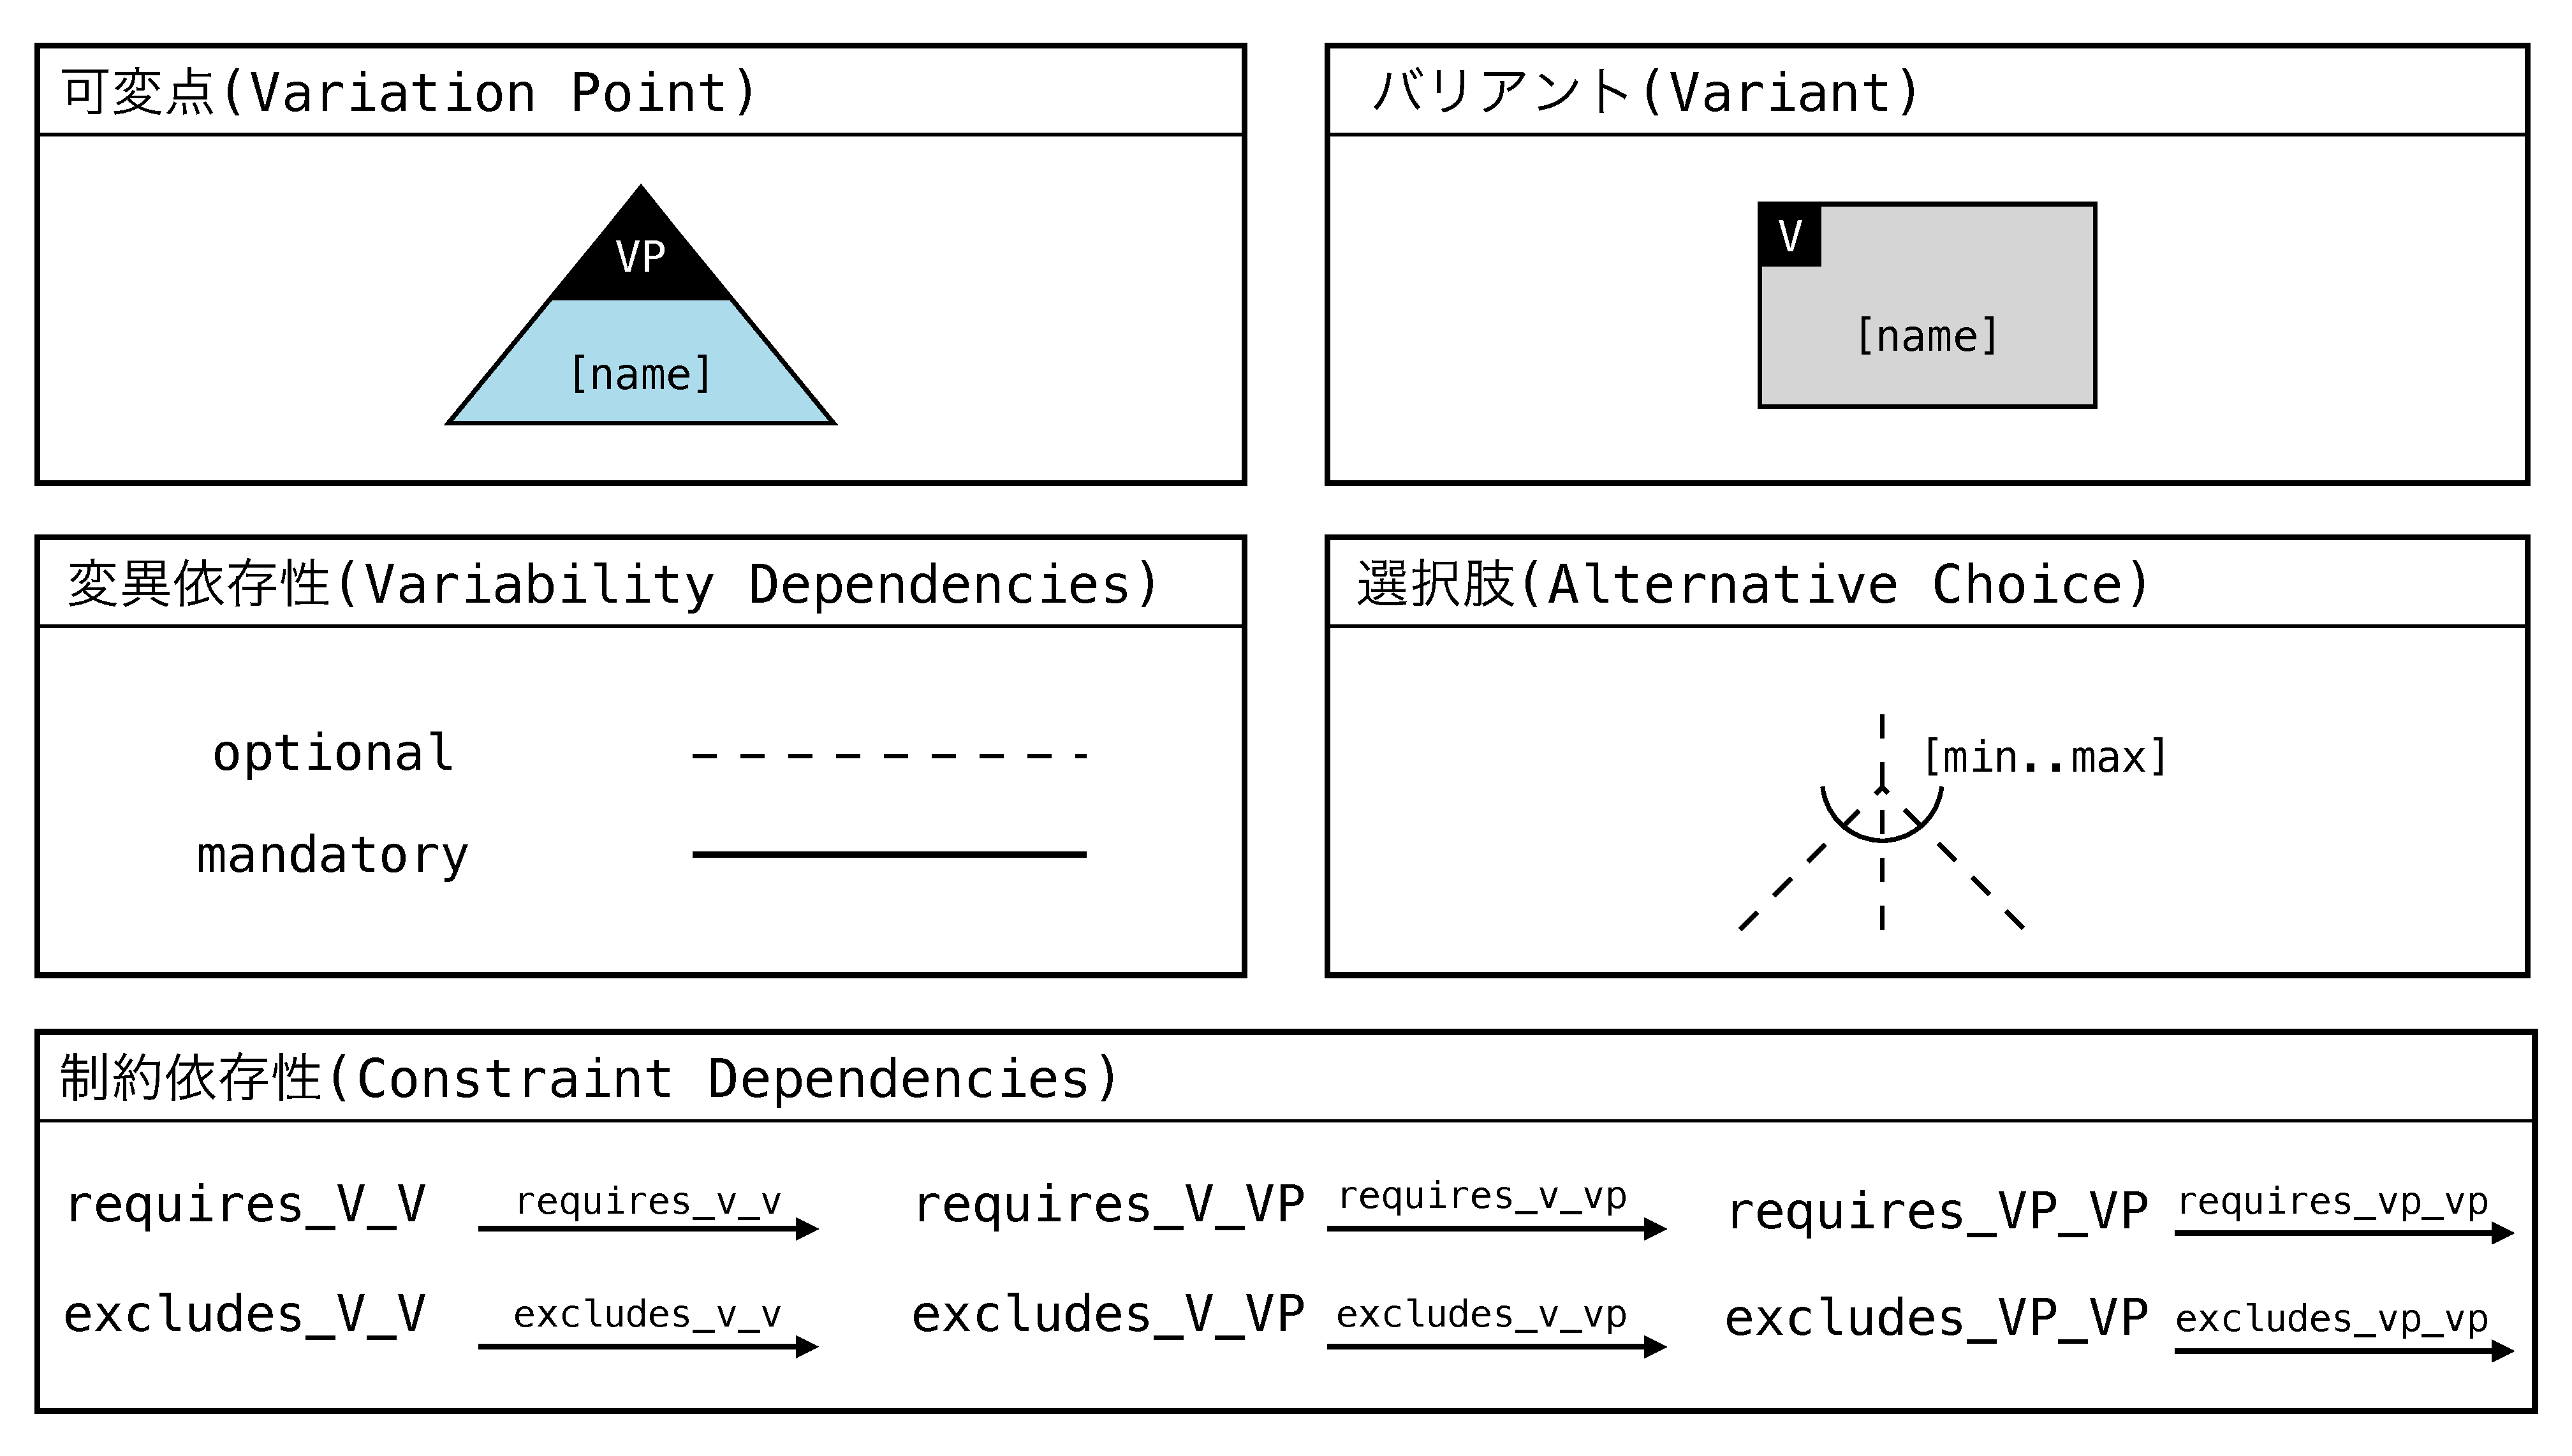
\includegraphics[width=\linewidth]{images/notation.eps}
  \caption{可変性モデルの表記法\cite{Pohl05:sple}}
  \label{fig:ovm_notation}
\end{figure}
%-------------------------------------------------------

CAFE問題の例を図~\ref{fig:ovm_example}に示す.
この例は,ソフトウェアプロダクトライン開発の分野で用いられる
\textbf{可変性モデル} (Orthogonal Variability Model; OVM\cite{Pohl05:sple})
によって記述されている.
図~\ref{fig:ovm_notation}に,可変性モデルの基本的な表記法を示す.
可変性モデルでは,
仕様ごとに変わりうる項目を\textbf{可変点}と呼び,三角形で表す.
可変点の具体的なインスタンスを\textbf{バリアント}と呼び,長方形で表す.
可変点とバリアントの対応関係には\textbf{変異依存性}と\textbf{選択肢}があり,
選択肢の場合は,その多重度も付記される.
可変点同士,バリアント同士,および,可変点とバリアント間の依存関係は,
\textbf{制約依存性}によって表される.
制約依存性には,要求(\textsf{requires})と排除(\textsf{excludes})の2種類がある.

可変性モデルでCAFE問題を記述する場合,
タイプは可変点,
オプションとその IWR 値はバリアント,
タイプとオプションの対応関係および
選択可能なオプション数の上下限値は選択肢,
タイプ同士,オプション同士,および,タイプとオプション間の依存関係は
制約依存性によって表される.
以上から,CAFE問題の入力のうち,
\ref{input:vp}〜\ref{input:iwr}は可変性モデルによって記述されるこ
とがわかる.

図~\ref{fig:ovm_example}の問題例は,
6個のタイプ,18個のオプション,5個の依存制約から構成され,
各タイプの選択可能なオプション数はすべて1である.
本論文では,可変点で表されるタイプは,各装備仕様に対して必須とする.
ただし,\textsf{Sun\_Roof}のような選択可能なタイプ(必須ではないタイプ)
については,破線の可変点で表すものとする.

%-------------------------------------------------------
\begin{table}[t]
  \centering
  \caption{CAFE問題(図~\ref{fig:ovm_example})の解}
  \begin{tabular}{l|l|c|c|c} \bhline
    %\multicolumn{1}{c|}{装備}   & \multicolumn{3}{c}{装備仕様} \\ \cline{2-4}
    \multicolumn{2}{l|}{装備仕様}               & 1	& 2 	 & 3	\\  \hline
    装備 & \textsf{Grade}        & \textsf{STD}    & \textsf{DX}     & \textsf{LX}\\
    &\textsf{Drive\_Type}  & \textsf{2WD}    & \textsf{2WD}    & \textsf{2WD}\\
    &\textsf{Engine}	  & \textsf{V4}     & \textsf{V6}     & \textsf{V6}\\
    &\textsf{Tire}	  & \textsf{16inch} & \textsf{17inch} & \textsf{18inch}\\
    &\textsf{Transmission} & \textsf{5MT}    & \textsf{6MT}    & \textsf{10AT}\\
    &\textsf{Sun\_Roof}    & -               & \textsf{Normal} & -  \\ \hline
    \multicolumn{2}{l|}{IWR 値の総和}           & 983  & 1,125   & 1,180 \\ %\hline
    \multicolumn{2}{l|}{燃費(km/L)}      & 10.2  & 8.9     & 8.5 \\ %\hline
    \multicolumn{2}{l|}{予想販売台数}    & 745   & 1,988   & 1,171  \\ \hline
    \multicolumn{2}{l|}{平均燃費(km/L)}  & \multicolumn{3}{c}{9.0} \\ 
    \multicolumn{2}{l|}{予想販売台数(合計)}  & \multicolumn{3}{c}{3,904} \\ \hline
 \end{tabular}
 \label{tab:ovm_ans}
\end{table}
%-------------------------------------------------------

図~\ref{fig:ovm_example}の問題に対する解の例を表\ref{tab:ovm_ans}に示す.
この解は,
CAFE 基準値に9.0km/L,
求めたい装備仕様の個数に3を与え,
装備仕様とオプションの依存関係として,
(装備仕様1, \textsf{STD}),
(装備仕様2, \textsf{DX}),
(装備仕様3, \textsf{LX})
を要求して得られたものである.
各装備仕様の燃費(km/L)は,左から順に 10.2, 8.9, 8.5 と
個々には CAFE 基準値を満たしていないが,
3台の平均燃費は 9.028km/L となり,CAFE 規制を満たしている.


%%% Local Variables:
%%% mode: japanese-latex
%%% TeX-master: "paper"
%%% End:

\section{解集合プログラミング} \label{chap:asp}

\textbf{解集合プログラミング} (Answer Set Programming; ASP~\cite{%
  Baral03:cambridge,%
  Gelfond88:iclp,%
  Inoue08:jssst,%
  Niemela99:amai})
は,演繹データベース,否定を含む論理プログラミング,
非単調推論,制約充足 (特に,SAT)を起源にもつ,
宣言的プログラミングパラダイムである.
ASP の言語は,一般拡張選言プログラムに基づいている.
本稿では説明の簡略化のため,そのサブクラスである
標準論理プログラムについて説明する.
以降,標準論理プログラムを単に論理プログラムとよぶ.

\textbf{論理プログラム}は,以下の形式をした\textbf{ルール}の有限集合である.
\[
  a_0\leftarrow a_1,\dots,a_m,\naf{a_{m+1}},\dots,\naf{a_n}
\]
ここで,
$0\leq m\leq n$ であり,
各$a_i$はアトム,
$\naf{}$はデフォルトの否定
\footnote{``失敗による否定''ともよばれる.述語論理で定義される否定($\neg$)とは意味が異なる.},
``$,$''は連言を表す.
$\leftarrow$の左側をヘッド,右側をボディとよぶ.
ルールの直観的な意味は,
「$a_1,\ldots,a_m$がすべて成り立ち,$a_{m+1},\ldots,a_n$のそれぞれが成
り立たないならば,$a_0$が成り立つ」である.
ボディが空のルール(すなわち\(a_0\leftarrow\))を\textbf{ファクト}とよび,
$\leftarrow$を省略してよい.

ヘッドが空のルールを\textbf{一貫性制約}とよぶ.
\[
  \leftarrow a_1,\dots,a_m,\naf{a_{m+1}},\dots,\naf{a_n}
\]

直観的には,\(\leftarrow a_1\)は,「$a_1$ではない」という禁止を表し,
\(\leftarrow \naf{a_1}\)は,「$a_1$でなければならない」という強制を表す.
また,
%\(\leftarrow a_1,a_2\)は,「$a_1$と$a_2$が両方同時に成り立つことはない」を意味し,
\(\leftarrow a_1, \naf{a_{2}}\)は,「$a_1$が成り立つならば,$a_2$が成り立つ」を意味する.

ASP 言語は,組合せ問題を解くための便利な拡張構文を備えている.
その代表的なものが\textbf{選択子}と\textbf{個数制約}である.
例えば,選択子\(\{a_1;\dots;a_n\}\)をファクトとして書くと,
「アトム集合\(\{a_1,\dots,a_n\}\)の任意の部分集合が成り立つ」を意味する.
個数制約は選択子の両端に選択可能な個数の上下限を付けたものである.
例えば,\(lb\ \{a_1;\dots;a_n\}\ ub \leftarrow Body\)と書くと,
「$Body$が成り立つならば,$a_1,\dots,a_n$のうち,$lb$個以上$ub$個以下
が成り立つ」を意味する.

\textbf{ASP システム}は,与えられた論理プログラムから,
安定モデル意味論~\cite{Gelfond88:iclp}
に基づく解集合を計算するソフトウェアである.
ASP システムの多くは,
変数を含む論理プログラムを変数を含まない論理プログラムに
\textbf{基礎化}したのち,基礎ソルバーを用いて解集合を計算する.
%近年,SAT ソルバー技術を応用した高速な ASP システムが開発されている.
本稿で使用する高速 ASP システム
{\clingo}~\footnote{\url{https://potassco.org/}}
は,基礎化のためのグラウンダー{\gringo}と基礎ソルバー{\clasp}を
シームレスに結合したものである.
以降で示す論理プログラムのソースコードはすべて{\clingo}言語で書か
れており,表記上の対応については表~\ref{tbl:map}の通りである.

%%%%%%%%%%%%%%%%%%%%%%%%%%%%%%%%%
\begin{table}[t]
  \centering
  \caption{論理プログラムとソースコードの対応}
  \tabcolsep = 2mm
  \begin{tabular}{l|*{5}{c}}\small
    論理プログラム &  $\leftarrow$ & $,$      & $;$      & $\sim$    \\\hline
    ソースコード   &  \code{:-}    & \code{,} & \code{;} & \code{not}
  \end{tabular}
  \label{tbl:map}
\end{table}
%%%%%%%%%%%%%%%%%%%%%%%%%%%%%%%%%
%%%%%%%%%%%%%%%%%%%%%%%%%%%%%%%%%
\lstinputlisting[float=t,caption={%
図~\ref{fig:graph}のグラフの ASP ファクト表現 (\code{graph.lp})},%
captionpos=b,frame=single,label=code:graph.lp,%
xrightmargin=1zw,% 
xleftmargin=1zw,% 
numbersep=5pt,%
numbers=none,%
breaklines=true,%
columns=fullflexible,keepspaces=true,%
basicstyle=\ttfamily\scriptsize]{code/graph.lp}
%%%%%%%%%%%%%%%%%%%%%%%%%%%%%%%%%
%%%%%%%%%%%%%%%%%%%%%%%%%%%%%%%%%
\lstinputlisting[float=t,caption={%
色数 \code{c} のグラフ点彩色問題を解く論理プログラム (\code{color.lp})},%
captionpos=b,frame=single,label=code:color.lp,%
xrightmargin=1zw,% 
xleftmargin=1zw,% 
numbersep=5pt,%
numbers=left,%
breaklines=true,%
columns=fullflexible,keepspaces=true,%
basicstyle=\ttfamily\scriptsize]{code/color.lp}
%%%%%%%%%%%%%%%%%%%%%%%%%%%%%%%%%
%%%%%%%%%%%%%%%%%%%%%%%%%%%%%%%%% 
\lstinputlisting[float=t,caption={%
{\clingo}の実行例},%
captionpos=b,frame=single,label=code:color.log,%
numbers=none,%
breaklines=true,%
columns=fullflexible,keepspaces=true,%
basicstyle=\ttfamily\scriptsize]{code/color.log}
%%%%%%%%%%%%%%%%%%%%%%%%%%%%%%%%%
%%%%%%%%%%%%%%%%%%%%%%%%%%%%%%%%%
\lstinputlisting[float=t,caption={%
基礎化された論理プログラム},%
captionpos=b,frame=single,label=code:color_ground.lp,%
xrightmargin=1zw,% 
xleftmargin=1zw,% 
numbersep=5pt,%
numbers=left,%
breaklines=true,%
columns=fullflexible,keepspaces=true,%
basicstyle=\ttfamily\scriptsize]{code/color_ground.lp}
%%%%%%%%%%%%%%%%%%%%%%%%%%%%%%%%%

ASP を用いた基本的な問題解法は,
最初に解きたい問題を論理プログラムとして表現する.
つぎにASP システムを用いて論理プログラムの解集合を計算する.
最後に解集合を解釈してもとの問題の解を得る,
という3つのステップからなる.
以下,グラフ点彩色問題を例にとって,各ステップごとに説明する.

図~\ref{fig:graph}の無向グラフを,ASP のファクト形式で表したものをコー
ド~\ref{code:graph.lp}に示す.
アトム\code{n/1}は頂点の数,
\code{e/1}は辺の数,
\code{node/1}は頂点,
\code{edge/2}は辺を表している.
ピリオド(``\code{.}'')はルールの終わりを表す終端記号である.

グラフ点彩色問題を解く論理プログラムを,
コード~\ref{code:color.lp}に示す.
コード中の\code{c}は色数を表す定数であり,実際の値は実行時に
{\clingo}のオプションとして与えられる.
1行目のアトム\code{col/1}は色を表し,
\code{col(1..c).}は\code{col(1).}, \code{col(2).}, \ldots,
\code{col(c).}と書くことに等しい.
%
2行目のルールは,頂点\code{X}が色\code{C}で塗られることを意
味するアトム\code{color(X,C)}を導入し,
個数制約を用いて「各頂点は1つの色で塗られる」という制約を表している.
% セミコロン(\code{:})は条件付きリテラ
% ルと呼ばれる拡張構文であり,このルールのヘッドは,
% \code{1 \{ color(X,r);color(X,b);color(X,g) \} 1}のように展開される.
3行目のルールは,一貫性制約と個数制約を使って「辺で結ばれた頂点\code{X}と
\code{Y}が同じ色\code{C}で塗られることはない」という制約を表している.

ASP システムは,
コード~\ref{code:graph.lp}のファクトと
コード~\ref{code:color.lp}の論理プログラム
から解集合を計算する.
コード~\ref{code:color.log}に{\clingo}の実行例を示す.
色\code{1}を赤,色\code{2}を青,色\code{3}を黄とすると,
得られた解集合\{
\code{color(1,1)},
\code{color(2,3)},
\code{color(3,1)},
\code{color(4,2)}\}
は,図~\ref{fig:graph}の右側の彩色を表す.
より詳しく言うと,
{\clingo}は,グラウンダー{\gringo}を用いて
コード~\ref{code:graph.lp}のファクトと
コード~\ref{code:color.lp}の論理プログラムを基礎化した後,
{\clasp}を用いて基礎化された論理プログラムの解集合を計算する.
基礎化されたルール集合をコード~\ref{code:color_ground.lp}に示す.
4--7行目が
コード~\ref{code:color.lp}の2行目に,
8--19行目が
コード~\ref{code:color.lp}の3行目に
対応している.

%%% Local Variables:
%%% mode: japanese-latex
%%% TeX-master: "paper"
%%% End:

%%%%%%%%%%%%%%%%%%%%%%%%%%%%%%%%%%%%%%%%%%%%%%%%%%%%%%%%%%
\chapter{クイーングラフ彩色問題のSMT符号化と$distinct$制約の高速化}
%%%%%%%%%%%%%%%%%%%%%%%%%%%%%%%%%%%%%%%%%%%%%%%%%%%%%%%%%%

本章ではSMTソルバーにおける$distinct$制約の高速化のために用いた手法についてそれぞれ述べる.
まず最初に,クイーングラフ彩色問題のSMT符号化について示し,次に高速化手法についてクイーングラフ彩色問題においてどのように表されるかを交えて説明を行う.

%%%%%%%%%%%%%%%%%%%%%%%%%%%%%%%%%%%%%%%%%%%%%%%%%%%%%%%%%%
%%
%% クイーングラフ彩色問題のSMT符号化
%%
%%%%%%%%%%%%%%%%%%%%%%%%%%%%%%%%%%%%%%%%%%%%%%%%%%%%%%%%%%
\section{クイーングラフ彩色問題のSMT符号化}
ここではN=5の場合のクイーングラフ彩色問題について使用したSMT符号化について説明する.
本研究ではチェス盤上の一番上の行を0行目,一番左の列を0列目とし,クイーンの色は整数として0から数えるものとする.


%%%%%%%%%%%%%%%%%%%%%%%%%%%%%%%%%%%%%%%%%%%%%%%%%%%%%%%%%%
\subsection{色変数モデルのSMT符号化}
%%%%%%%%%%%%%%%%%%%%%%%%%%%%%%%%%%%%%%%%%%%%%%%%%%%%%%%%%%
まず,整数変数c\_0\_0は以下のように宣言される.
c\_i\_jはi行j列目のクイーンの色を示している.
{ \scriptsize \begin{verbatim}
    (declare-const c_0_0 Int)
\end{verbatim}}
また,c\_0\_0は0以上4以下であるので以下の制約を追加する.
{ \scriptsize \begin{verbatim}
    (assert (and (>= c_0_0 0) (<= c_0_0 4)))
\end{verbatim}}
他の変数についても同様に宣言される.

次に,0行目に配置されるクイーンの色が互いに異なるという制約は以下のように宣言される.
{ \scriptsize \begin{verbatim}
    (assert (distinct c_0_0 c_0_1 c_0_2 c_0_3 c_0_4)))
\end{verbatim}}
他の行や列,右上がり対角線や右下がり対角線についても同様に宣言される.


作成したN=5の場合の色変数モデルのコードをコード\ref{code:qgcp_5_col}に示す.
3から52行目が各整数変数の宣言とそのドメインを指定しており,
53から57行目が各行についての制約であり,
58から62行目が各列について,
63から69行目が各右上がり対角線について,
70から76行目が角右下がり対角線についてである.
また,77から81行目は対称性除去のために0行目の値を指定している.

\lstinputlisting[float=htbp,caption={%
N=5の色変数モデルのクイーングラフ彩色問題},%
captionpos=b,frame=single,label=code:qgcp_5_col,%
numbers=left,%
breaklines=true,%
columns=fullflexible,keepspaces=true,%
basicstyle=\ttfamily\tiny]{code/qgcp_5_m0__z3_489.smt2}


%%%%%%%%%%%%%%%%%%%%%%%%%%%%%%%%%%%%%%%%%%%%%%%%%%%%%%%%%%
\subsection{位置変数モデルのSMT符号化}
%%%%%%%%%%%%%%%%%%%%%%%%%%%%%%%%%%%%%%%%%%%%%%%%%%%%%%%%%%
まず,整数変数y\_0\_0は以下のように宣言される.
y\_i\_kはi行目のk色のクイーンが配置される場所を示している.
{ \scriptsize \begin{verbatim}
    (declare-const y_0_0 Int)
\end{verbatim}}
また,y\_0\_0は0以上4以下であるので以下の制約を追加する.
{ \scriptsize \begin{verbatim}
    (assert (and (>= y_0_0 0) (<= y_0_0 4)))
\end{verbatim}}
他の変数についても同様に宣言される.

次に,0行目に配置される5色のクイーンがそれぞれ異なる列に配置されるという制約は以下のように宣言される.
{ \scriptsize \begin{verbatim}
    (assert (distinct y_0_0 y_0_1 y_0_2 y_0_3 y_0_4)))
\end{verbatim}}
他の行や列についても同様に宣言される.

右上がり対角線について,色0が配置される行と列の和が2つ以上同じにならないという制約は以下のように宣言される.
{ \scriptsize \begin{verbatim}
    (assert (distinct (+ y_0_0 0) (+ y_1_0 1) (+ y_2_0 2) (+ y_3_0 3) (+ y_4_0 4)))
\end{verbatim}}
他の色についても同様に宣言される.

右下がり対角線について,色0が配置される行と列の差が2つ以上同じにならないという制約は以下のように宣言される.
{ \scriptsize \begin{verbatim}
    (assert (distinct (- y_0_0 0) (- y_1_0 1) (- y_2_0 2) (- y_3_0 3) (- y_4_0 4)))
\end{verbatim}}
他の色についても同様に宣言される.


作成したN=5の場合の位置変数モデルのコードを\ref{code:qgcp_5_pos}に示す.
色変数モデルの時と同様にして,
3から52行目が各整数変数の宣言とそのドメインを指定しており,
53から72行目が各行,各列,各右上がり対角線,各右下がり対角線についてそれぞれ互いに異なるという制約を追加している.
また,73から77行目は対称性除去のために0行目に配置されるクイーンの列を指定して宣言している.

\lstinputlisting[float=htbp,caption={%
N=5の位置変数モデルのクイーングラフ彩色問題},%
captionpos=b,frame=single,label=code:qgcp_5_pos,%
numbers=left,%
breaklines=true,%
columns=fullflexible,keepspaces=true,%
basicstyle=\ttfamily\tiny]{code/qgcp_5_m7__z3_489.smt2}


%%%%%%%%%%%%%%%%%%%%%%%%%%%%%%%%%%%%%%%%%%%%%%%%%%%%%%%%%%
\subsection{0-1変数モデルのSMT符号化}\label{sec:pro_pb}
%%%%%%%%%%%%%%%%%%%%%%%%%%%%%%%%%%%%%%%%%%%%%%%%%%%%%%%%%%

% 高速化のための2つ目の手法は$distinct$制約をPB符号化して解くというものである.
% この手法では,求める解を整数変数としてではなく0-1変数として求める.
%
% 例としては,整数変数$x \in \{1,2,3\}$は0-1変数$x_1,x_2,x_3 \in {0,1}$として,$x_i=1$なら$x=i$というようにして解を求める.
%
% N=5の場合について本研究で使用したSMT符号化を説明する
まず,0-1変数c\_0\_0\_0は以下のように宣言される.
c\_i\_j\_kはi行j列目がk色に塗られるかどうかを示している.
{ \scriptsize \begin{verbatim}
    (declare-const c_0_0_0 Int)
\end{verbatim}}
また,c\_0\_0\_0は0-1変数であるので以下の制約を追加する.
{ \scriptsize \begin{verbatim}
    (assert (and (>= c_0_0_0 0) (<= c_0_0_0 1)))
\end{verbatim}}
他の変数についても同様に宣言される.
盤面上の一つのマスに塗られる色は一色だけなので,0行0列目が一つの色で塗られる制約は以下のようになる.
{ \scriptsize \begin{verbatim}
(assert (= (+ c_0_0_0 c_0_0_1 c_0_0_2 c_0_0_3 c_0_0_4) 1))
\end{verbatim}}
他のマスについても同様に宣言される.この制約は式\ref{eq:smt_pb_1}に対応しており,重複を避けるためにまとめて宣言する.

次に,0行目に配置されるクイーンの色が互いに異なるという制約は以下のように宣言される.
{ \scriptsize \begin{verbatim}
(assert (= (+ c_0_0_0 c_0_1_0 c_0_2_0 c_0_3_0 c_0_4_0) 1))
(assert (= (+ c_0_0_1 c_0_1_1 c_0_2_1 c_0_3_1 c_0_4_1) 1))
(assert (= (+ c_0_0_2 c_0_1_2 c_0_2_2 c_0_3_2 c_0_4_2) 1))
(assert (= (+ c_0_0_3 c_0_1_3 c_0_2_3 c_0_3_3 c_0_4_3) 1))
(assert (= (+ c_0_0_4 c_0_1_4 c_0_2_4 c_0_3_4 c_0_4_4) 1))
\end{verbatim}}
他の行や列についても同様に宣言される.

右上がり対角線について,\verb|c_0_3, c_1_2, c_2_1, c_3_0|が互いに異なるという制約は以下のように宣言される.
{ \scriptsize \begin{verbatim}
(assert (<= (+ c_0_3_0 c_1_2_0 c_2_1_0 c_3_0_0) 1))
(assert (<= (+ c_0_3_1 c_1_2_1 c_2_1_1 c_3_0_1) 1))
(assert (<= (+ c_0_3_2 c_1_2_2 c_2_1_2 c_3_0_2) 1))
(assert (<= (+ c_0_3_3 c_1_2_3 c_2_1_3 c_3_0_3) 1))
(assert (<= (+ c_0_3_4 c_1_2_4 c_2_1_4 c_3_0_4) 1))
\end{verbatim}}
他の右上がり対角線についても同様に宣言されるが,$i+j=N-1$の場合は上記の\verb|<=|は\verb|=|に変更して以下のように宣言される.
{ \scriptsize \begin{verbatim}
(assert (= (+ c_0_4_0 c_1_3_0 c_2_2_0 c_3_1_0 c_4_0_0) 1))
(assert (= (+ c_0_4_1 c_1_3_1 c_2_2_1 c_3_1_1 c_4_0_1) 1))
(assert (= (+ c_0_4_2 c_1_3_2 c_2_2_2 c_3_1_2 c_4_0_2) 1))
(assert (= (+ c_0_4_3 c_1_3_3 c_2_2_3 c_3_1_3 c_4_0_3) 1))
(assert (= (+ c_0_4_4 c_1_3_4 c_2_2_4 c_3_1_4 c_4_0_4) 1))
\end{verbatim}}
右下がり対角線については$i-j=N-1$の場合に\verb|<=|を\verb|=|に変更し同様にして宣言される.


作成したN=5の場合の色変数モデルのコードをコード\ref{code:qgcp_5_pb}に示す.
3から277行目が各整数変数の宣言とそのドメインと色の制約を追加しており,
278から425行目が各行,各列,各右上がり対角線,各右下がり対角線についてそれぞれ互いに異なるという制約を追加している.
また,426から430行目は対称性除去のために0行目の値を指定している.

\begin{lstlisting}[frame=trl,numbers=left,breaklines=true,%
columns=fullflexible,keepspaces=true,%
basicstyle=\ttfamily\scriptsize]
; QGCP model=18 n=5 opts={'-m': '18', '-x': ''}
; color-variable model (pb)
(declare-const c_0_0_0 Int)
(assert (and (>= c_0_0_0 0) (<= c_0_0_0 1)))
(declare-const c_0_0_1 Int)
(assert (and (>= c_0_0_1 0) (<= c_0_0_1 1)))
(declare-const c_0_0_2 Int)
(assert (and (>= c_0_0_2 0) (<= c_0_0_2 1)))
(declare-const c_0_0_3 Int)
(assert (and (>= c_0_0_3 0) (<= c_0_0_3 1)))
(declare-const c_0_0_4 Int)
(assert (and (>= c_0_0_4 0) (<= c_0_0_4 1)))
(declare-const c_0_1_0 Int)
(assert (and (>= c_0_1_0 0) (<= c_0_1_0 1)))
(declare-const c_0_1_1 Int)
(assert (and (>= c_0_1_1 0) (<= c_0_1_1 1)))
(declare-const c_0_1_2 Int)
(assert (and (>= c_0_1_2 0) (<= c_0_1_2 1)))
(declare-const c_0_1_3 Int)
(assert (and (>= c_0_1_3 0) (<= c_0_1_3 1)))
(declare-const c_0_1_4 Int)
(assert (and (>= c_0_1_4 0) (<= c_0_1_4 1)))
(declare-const c_0_2_0 Int)
(assert (and (>= c_0_2_0 0) (<= c_0_2_0 1)))
(declare-const c_0_2_1 Int)
(assert (and (>= c_0_2_1 0) (<= c_0_2_1 1)))
(declare-const c_0_2_2 Int)
(assert (and (>= c_0_2_2 0) (<= c_0_2_2 1)))
(declare-const c_0_2_3 Int)
(assert (and (>= c_0_2_3 0) (<= c_0_2_3 1)))
(declare-const c_0_2_4 Int)
(assert (and (>= c_0_2_4 0) (<= c_0_2_4 1)))
(declare-const c_0_3_0 Int)
(assert (and (>= c_0_3_0 0) (<= c_0_3_0 1)))
(declare-const c_0_3_1 Int)
(assert (and (>= c_0_3_1 0) (<= c_0_3_1 1)))
(declare-const c_0_3_2 Int)
(assert (and (>= c_0_3_2 0) (<= c_0_3_2 1)))
(declare-const c_0_3_3 Int)
(assert (and (>= c_0_3_3 0) (<= c_0_3_3 1)))
(declare-const c_0_3_4 Int)
(assert (and (>= c_0_3_4 0) (<= c_0_3_4 1)))
(declare-const c_0_4_0 Int)
(assert (and (>= c_0_4_0 0) (<= c_0_4_0 1)))
(declare-const c_0_4_1 Int)
(assert (and (>= c_0_4_1 0) (<= c_0_4_1 1)))
(declare-const c_0_4_2 Int)
(assert (and (>= c_0_4_2 0) (<= c_0_4_2 1)))
(declare-const c_0_4_3 Int)
(assert (and (>= c_0_4_3 0) (<= c_0_4_3 1)))
(declare-const c_0_4_4 Int)
(assert (and (>= c_0_4_4 0) (<= c_0_4_4 1)))
\end{lstlisting}
$\vdots$
\begin{lstlisting}[frame=rl,numbers=left,breaklines=true,%
columns=fullflexible,keepspaces=true,%
basicstyle=\ttfamily\scriptsize,firstnumber=253]
(assert (= (+ c_0_0_0 c_0_0_1 c_0_0_2 c_0_0_3 c_0_0_4) 1))
(assert (= (+ c_0_1_0 c_0_1_1 c_0_1_2 c_0_1_3 c_0_1_4) 1))
(assert (= (+ c_0_2_0 c_0_2_1 c_0_2_2 c_0_2_3 c_0_2_4) 1))
(assert (= (+ c_0_3_0 c_0_3_1 c_0_3_2 c_0_3_3 c_0_3_4) 1))
(assert (= (+ c_0_4_0 c_0_4_1 c_0_4_2 c_0_4_3 c_0_4_4) 1))
\end{lstlisting}
$\vdots$

\begin{lstlisting}[frame=rl,numbers=left,breaklines=true,%
columns=fullflexible,keepspaces=true,%
basicstyle=\ttfamily\scriptsize,firstnumber=278]
; alldiff_pb c_0_0 c_0_1 c_0_2 c_0_3 c_0_4
(assert (= (+ c_0_0_0 c_0_1_0 c_0_2_0 c_0_3_0 c_0_4_0) 1))
(assert (= (+ c_0_0_1 c_0_1_1 c_0_2_1 c_0_3_1 c_0_4_1) 1))
(assert (= (+ c_0_0_2 c_0_1_2 c_0_2_2 c_0_3_2 c_0_4_2) 1))
(assert (= (+ c_0_0_3 c_0_1_3 c_0_2_3 c_0_3_3 c_0_4_3) 1))
(assert (= (+ c_0_0_4 c_0_1_4 c_0_2_4 c_0_3_4 c_0_4_4) 1))
\end{lstlisting}
$\vdots$

\begin{lstlisting}[frame=rbl,numbers=left,breaklines=true,%
columns=fullflexible,keepspaces=true,%
basicstyle=\ttfamily\scriptsize,firstnumber=426,%
captionpos=b,caption={N=5の0-1変数のみを用いた色変数モデルのクイーングラフ彩色問題},label={code:qgcp_5_pb}]
(assert (= c_0_0_0 1))
(assert (= c_0_1_1 1))
(assert (= c_0_2_2 1))
(assert (= c_0_3_3 1))
(assert (= c_0_4_4 1))
(check-sat)
(get-model)
(exit)
\end{lstlisting}


% \lstinputlisting[float=htbp,caption={%
% N=5の0-1変数のみを用いた色変数モデルのクイーングラフ彩色問題},%
% captionpos=b,frame=single,label=code:qgcp_5_pb,%
% numbers=left,%
% classoffset=1,%
% breaklines=true,%
% columns=fullflexible,keepspaces=true,%
% basicstyle=\ttfamily\tiny]{code/qgcp_5_m18__z3_489.smt2}

% 本研究では,$distinct$制約を3つ方法で符号化した.
% これらは,参考文献\cite{Ono19:ai}から引用したものであり,
% % 1つ目はブール基数制約符号化のみを使用したもので\ref{sec:pb4smt}に示したものである,2つ目と3つ目はブール基数制約符号化にヒント制約を追加したものである.
% 1つ目はat-most-one制約を用いてdistinct制約を表したもので,2つ目はと3つ目は新たに変数を導入することでヒントを追加し,distinct制約を表すものである.
%
%
% %\subsection{符号化方法1}\label{sec:pb_1}
% 1つ目の符号化は$distinct$制約を以下のように表すものである.
%
% $distinct(x_1 ... x_n)$について,$x_i$は1以上$d$以下の値で$n \leq d$とし,
% $x_{ij}$は$x_{ij} = 1 \leftrightarrow x_i = j$であるとすると,
% \begin{eqnarray}
%     x_{i1} + ... + x_{id}=1 \; (i=1 ... n) \label{eq:pb_1_1}\\
%     x_{1j} + ... + x_{nj}\leq1 \; (j=1 ... d) \label{eq:pb_1_2}
% \end{eqnarray}
% (\ref{eq:pb_1_1})は$x_i$がちょうど1つの値しか取らないことを表し,
% (\ref{eq:pb_1_2})は各値$j$が割り当て割れるのが高々1つの変数であることを表している.
%
% また,$n=d$の時,(\ref{eq:pb_1_2})は以下の制約に置き換えられる.
% \begin{eqnarray}
%     x_{1j} + ... + x_{nj}=1 \; (j=1 ... d) \label{eq:pb_1_3}
% \end{eqnarray}
% これは各値jがちょうど1つの変数に割り当てられることを表している.
%
% これらの制約についてSMT符号化を行うと,
% 例として,N=5の時に\verb|(distinct c_0_0 c_0_1 c_0_2 c_0_3 c_0_4)|は以下のように宣言される.
%
% { \scriptsize \begin{verbatim}
% (assert (= (+ c_0_0_0 c_0_0_1 c_0_0_2 c_0_0_3 c_0_0_4) 1))
% (assert (= (+ c_0_1_0 c_0_1_1 c_0_1_2 c_0_1_3 c_0_1_4) 1))
% (assert (= (+ c_0_2_0 c_0_2_1 c_0_2_2 c_0_2_3 c_0_2_4) 1))
% (assert (= (+ c_0_3_0 c_0_3_1 c_0_3_2 c_0_3_3 c_0_3_4) 1))
% (assert (= (+ c_0_4_0 c_0_4_1 c_0_4_2 c_0_4_3 c_0_4_4) 1))
% (assert (= (+ c_1_0_0 c_1_0_1 c_1_0_2 c_1_0_3 c_1_0_4) 1))
% (assert (= (+ c_0_0_0 c_0_1_0 c_0_2_0 c_0_3_0 c_0_4_0) 1))
% (assert (= (+ c_0_0_1 c_0_1_1 c_0_2_1 c_0_3_1 c_0_4_1) 1))
% (assert (= (+ c_0_0_2 c_0_1_2 c_0_2_2 c_0_3_2 c_0_4_2) 1))
% (assert (= (+ c_0_0_3 c_0_1_3 c_0_2_3 c_0_3_3 c_0_4_3) 1))
% (assert (= (+ c_0_0_4 c_0_1_4 c_0_2_4 c_0_3_4 c_0_4_4) 1))
% \end{verbatim}}


%%%%%%%%%%%%%%%%%%%%%%%%%%%%%%%%%%%%%%%%%%%%%%%%%%%%
%
% ヒント制約の追加
%
%%%%%%%%%%%%%%%%%%%%%%%%%%%%%%%%%%%%%%%%%%%%%%%%%%%%
\section{$distinct$制約の高速化}\label{sec:pro_hint}

高速化のための手法として3つの手法を用いた.
% 高速化のための手法の1つ目は$distinct$制約にヒント制約を追加することである.
% 追加したヒント制約は2つあり,1つは鳩の巣原理を用いたヒント制約で,もう一つはat-most-one制約を用いたヒント制約である.

\subsection{鳩の巣原理を用いたヒント制約}\label{sec:pro_hint_1}
1つ目の手法は鳩の巣原理を用いたヒント制約の追加である.
このヒント制約は参考文献\cite{Tamura:queen}から引用したものであり,追加した制約は以下の通りである.
% 1つ目の鳩の巣原理を用いたヒント制約は,参考文献\cite{Tamura:queen}から引用したものであり,追加した制約は以下の通りである,

$distinct(x_1 ... x_n)$について,$x_i \in \{l, l+1, ..., u\}$であるとき
\begin{eqnarray}
&& \bigvee_{i=1}^n   x_i \geq l+n-1\\
\label{eq:pro_h1_1}
&& \bigvee_{i=1}^n \lnot(x_i \geq u-n+1)
\label{eq:pro_h1_2}
\end{eqnarray}
である.

(\ref{eq:pro_h1_1})は,全ての$x_i$が$l+n-2$以下になることを禁止しており,
(\ref{eq:pro_h1_2})は,全ての$x_i$が$u-n+1$以上になることを禁止している.

この制約についてSMT符号化を行うと.
例として,N=5での時に\\
\verb|(distinct c_0_3 c_1_2 c_2_1 c_3_0)|は以下のように宣言される.

% \begin{framed}
{ \scriptsize \begin{verbatim}
(assert (distinct c_0_3 c_1_2 c_2_1 c_3_0))
(assert (or (>= c_0_3 3) (>= c_1_2 3) (>= c_2_1 3) (>= c_3_0 3)))
(assert (or (<= c_0_3 1) (<= c_1_2 1) (<= c_2_1 1) (<= c_3_0 1)))
\end{verbatim}}
% \end{framed}

この制約を追加する利点としては,
上記の例においては,c\_0\_3,c\_1\_2,c\_2\_1がそれぞれ0,1,2の値を取るとしたときに,c\_3\_0の取り得る範囲が3以上4以下に制限される.
このように,制限を加わえることができるので,探索範囲が狭まり求解速度を上げることができる.


\subsection{at-least-one 制約を用いたヒント制約}\label{sec:pro_hint_2}
2つ目の手法は,$distinct$制約の要素のドメインのサイズと要素数が等しい場合,つまり
$distinct(x_1 ... x_n)$について,$x_i \in \{l, l+1, ..., u\}$かつ$u-l=n-1$であるときに以下の制約を追加するものである.\\
\begin{eqnarray}
\bigvee_{i=1}^n x_i=a \; (a \in \{l, l+1, ..., u\})
\label{eq:pro_h2}
\end{eqnarray}
この制約はドメインサイズと要素数が等しい場合には,値$a$に対してその値をとる変数$x_i$が存在するというヒントを追加している.

この制約についてSMT符号化を行うと.
例として,N=5の時に\\
\verb|(distinct c_0_0 c_0_1 c_0_2 c_0_3 c_0_4)|は以下のように宣言される.

{ \scriptsize \begin{verbatim}
(assert (distinct c_0_0 c_0_1 c_0_2 c_0_3 c_0_4))
(assert (or (= c_0_0 0) (= c_0_1 0) (= c_0_2 0) (= c_0_3 0) (= c_0_4 0)))
(assert (or (= c_0_0 1) (= c_0_1 1) (= c_0_2 1) (= c_0_3 1) (= c_0_4 1)))
(assert (or (= c_0_0 2) (= c_0_1 2) (= c_0_2 2) (= c_0_3 2) (= c_0_4 2)))
(assert (or (= c_0_0 3) (= c_0_1 3) (= c_0_2 3) (= c_0_3 3) (= c_0_4 3)))
(assert (or (= c_0_0 4) (= c_0_1 4) (= c_0_2 4) (= c_0_3 4) (= c_0_4 4)))
\end{verbatim}}


この制約を追加する利点としては,
上記の例においては,探索を進めていくにつれてc\_0\_0,c\_0\_1,c\_0\_2,c\_0\_3,c\_0\_4が0にならないと分かった時点でその解が間違っているとわかるので枝刈りを行うことができ,
求解速度を上げることができる.


\subsection{$distinct$制約のPB符号化を用いた改良}\label{sec:pro_hint_3}
3つ目の手法は$distinct$制約のPB符号化に改良を加えるものである.
これは参考文献\cite{Ono19:ai}から引用したものであり,2つの改良手法を用いた.


\subsubsection{改良手法1}\label{sec:pro_hint_3_1}
1つ目の改良手法は$distinct$制約のPB符号化を以下のように表すものである.

$distinct(x_1 ... x_n)$について,$n < d$の時,
各値$j$ごとの$x_{ij}$の和を表す変数$y_j$を導入し,以下のように表す.
\begin{eqnarray}
    x_{i1} + ... + x_{id}=1 \; (i=1 ... n) \label{eq:pro_pb_1_1}\\
    x_{1j} + ... + x_{nj}\leq1 \; (j=1 ... d) \label{eq:pro_pb_1_2}\\
    y_j = x_{1j} + ... + x_{nj} \; (j=1 ... d) \label{eq:pro_pb_1_3}\\
    y_1 + ... + y_d =n \label{eq:pro_pb_1_4}
\end{eqnarray}

(\ref{eq:pro_pb_1_3})(\ref{eq:pro_pb_1_4})についてSMT符号化を行うと,
例として,N=5での時に\verb|(distinct c_0_1 c_1_0)|は以下のように宣言される.

{ \scriptsize \begin{verbatim}
(declare-const _T1_0 Int)
(assert (and (>= _T1_0 0) (<= _T1_0 1)))
(declare-const _T1_1 Int)
(assert (and (>= _T1_1 0) (<= _T1_1 1)))
(declare-const _T1_2 Int)
(assert (and (>= _T1_2 0) (<= _T1_2 1)))
(declare-const _T1_3 Int)
(assert (and (>= _T1_3 0) (<= _T1_3 1)))
(declare-const _T1_4 Int)
(assert (and (>= _T1_4 0) (<= _T1_4 1)))
(assert (= _T1_0 (+ c_0_1_0 c_1_0_0)))
(assert (= _T1_1 (+ c_0_1_1 c_1_0_1)))
(assert (= _T1_2 (+ c_0_1_2 c_1_0_2)))
(assert (= _T1_3 (+ c_0_1_3 c_1_0_3)))
(assert (= _T1_4 (+ c_0_1_4 c_1_0_4)))
(assert (= (+ _T1_0 _T1_1 _T1_2 _T1_3 _T1_4) 2))
\end{verbatim}}

この制約を追加する利点としては,
上記の例においては,探索を進めていくにつれて
c\_0\_1,c\_1\_0が1,2,3,4にならないと分かった時点では,\ref{eq:pro_pb_1_1}と\ref{eq:pro_pb_1_2}の制約には違反しないが,
{\small \verb|_T1_0 + _T1_1 + _T1_2 + _T1_3 + _T1_4 = 2| }が成り立たないことがわかるため
枝刈りを行うことができ,求解速度を上げることができる.

%\subsection{符号化方法3}
\subsubsection{改良手法2}\label{sec:pro_hint_3_2}
1つ目の改良手法は$distinct$制約のPB符号化を以下のように表すものである.
2つ目の改良手法は$distinct$制約を以下のように表すものである.

$distinct(x_1 ... x_n)$について,$n < d$の時,
各値$j$ごとに新たな変数$x_{(n+1)j}$を導入し,以下のように表す.
\begin{eqnarray}
    x_{i1} + ... + x_{id}=1 \; (i=1 ... n) \label{eq:pro_pb_2_1}\\
    x_{(n+1)1} + ... + x_{(n+1)d}=d-n \label{eq:pro_pb_2_2}\\
    x_{1j} + ... + x_{(n+1)j}=1 \; (j=1 ... d) \label{eq:pro_pb_2_3}\\
\end{eqnarray}

(\ref{eq:pro_pb_2_2})(\ref{eq:pro_pb_2_3})についてSMT符号化を行うと,
例として,N=5での時に\verb|(distinct c_0_1 c_1_0)|は以下のように宣言される.

{ \scriptsize \begin{verbatim}
(declare-const _T1_0 Int)
(assert (and (>= _T1_0 0) (<= _T1_0 1)))
(declare-const _T1_1 Int)
(assert (and (>= _T1_1 0) (<= _T1_1 1)))
(declare-const _T1_2 Int)
(assert (and (>= _T1_2 0) (<= _T1_2 1)))
(declare-const _T1_3 Int)
(assert (and (>= _T1_3 0) (<= _T1_3 1)))
(declare-const _T1_4 Int)
(assert (and (>= _T1_4 0) (<= _T1_4 1)))
(assert (= (+ _T1_0 _T1_1 _T1_2 _T1_3 _T1_4) 3))
(assert (= (+ c_0_1_0 c_1_0_0 _T1_0) 1))
(assert (= (+ c_0_1_1 c_1_0_1 _T1_1) 1))
(assert (= (+ c_0_1_2 c_1_0_2 _T1_2) 1))
(assert (= (+ c_0_1_3 c_1_0_3 _T1_3) 1))
(assert (= (+ c_0_1_4 c_1_0_4 _T1_4) 1))
\end{verbatim}}

この制約を追加する利点としては,
上記の例においては,探索を進めていくにつれて
c\_0\_1,c\_1\_0が1,2,3,4にならないと分かった時点では,\ref{eq:pro_pb_2_1}の制約には違反しないが,
{\small \verb|_T1_0 + _T1_1 + _T1_2 + _T1_3 + _T1_4 = 3|}が成り立たないことがわかるため
枝刈りを行うことができ,求解速度を上げることができる.



%%%%%%%%%%%%%%%%%%%%%%%%%%%%%%%%%%%%%%%%%%%%%%%%%%%%
%
% チャネリング
%
%%%%%%%%%%%%%%%%%%%%%%%%%%%%%%%%%%%%%%%%%%%%%%%%%%%%
\section{チャネリング制約を用いたクイーングラフ彩色問題のSMT符号化}\label{sec:pro_pb_c}
\ref{sec:pro_hint_3}に示した高速化手法は\ref{sec:bg_pb}の0-1変数モデルに対してのみ用いることができる.
整数変数を用いている色変数モデルと位置変数モデルに対してもこの高速化手法を実装するためにチャネリング制約を用いた.

この手法では求める解は整数変数として求めるが,$distinct$制約を解く際にチャネリング制約を追加し求める整数変数を0-1変数に変換してからPB符号化で解く.

N=5の時,c\_0\_0について追加したチャネリング制約は以下のものである.
{ \scriptsize \begin{verbatim}
(assert (=> (= c_0_0_0 1) (= c_0_0 0)))
(assert (=> (= c_0_0 0) (= c_0_0_0 1)))
(assert (=> (= c_0_0_1 1) (= c_0_0 1)))
(assert (=> (= c_0_0 1) (= c_0_0_1 1)))
(assert (=> (= c_0_0_2 1) (= c_0_0 2)))
(assert (=> (= c_0_0 2) (= c_0_0_2 1)))
(assert (=> (= c_0_0_3 1) (= c_0_0 3)))
(assert (=> (= c_0_0 3) (= c_0_0_3 1)))
(assert (=> (= c_0_0_4 1) (= c_0_0 4)))
(assert (=> (= c_0_0 4) (= c_0_0_4 1)))
\end{verbatim}}
これは
\begin{eqnarray}
    c_{ijk} = 1 \Leftrightarrow c_{ij} = k
\end{eqnarray}
を表す.
他の変数に対しても同様に宣言される.また,$distinct$制約を扱う際には\verb|c_i_j_k|を用いて制約が生成される.


% この手法の利点としては上記\ref{sec:pb}の手法では$distinct$制約の要素に式が存在する場合,新たに変数を導入して

%%% Local Variables:
%%% mode: latex
%%% TeX-master: "paper"
%%% End:

%%%%%%%%%%%%%%%%%%%%%%%%%%%%%%%%%%%%%%%%%%%%%%%%%%%%%%%%%% 
\section{実行実験}\label{chap:experiment}
%%%%%%%%%%%%%%%%%%%%%%%%%%%%%%%%%%%%%%%%%%%%%%%%%%%%%%%%%% 

本章では,前章で提案した3つの符号化
\textsf{undirected},\textsf{directed},\textsf{acyclicity}
の性能を評価するために実行実験を行った.
%
実験に使用したベンチマーク問題集(計1008問)は,以下の通りである.
\begin{itemize}
\item \textsf{fhcp} (1001問)\\
  Jerzy Filar と Vladimir Ejov が主導する
  チームプロジェクト Flinders Hamiltonian Cycle Project
  \footnote{\url{https://sites.flinders.edu.au/flinders-hamiltonian-cycle-project/}}
  が提供するハミルトン閉路問題のグラフインスタンス.\cite{haythorpe19:fhcp}
\item \textsf{grid} (6問)\\
  $2N+1$次の正方グリッドグラフのインスタンス($3\leq N\leq 8$).
\item \textsf{usmap} (1問)\\
  図~\ref{fig:USmap}に示されたグラフ.
  D.~E~.Knuth の教科書
  The Art of Computer Programming~\cite{Knuth:TAOCP:SAT}
  に記載されている最短ハミルトン路問題の例.
\end{itemize}

使用した ASP システムは{\clingo}のバージョン5.5.0である.
実験環境は,Mac mini Intel Corei7 3.2GHz 64GBメモリである.

%%%%%%%%%%%%%%%%%%%%%%%%%%%%%%%%%%%%%%%%%%%%%%%%%%%%%%%%%%
\subsection{ハミルトン閉路問題の実験結果}
%%%%%%%%%%%%%%%%%%%%%%%%%%%%%%%%%%%%%%%%%%%%%%%%%%%%%%%%%%

%%%%%%%%%%%%%%%%%%%%%%%%%%%%%%%%%%%%%%%%%%%%%%%
\begin{table}[t]\scriptsize
  \centering
  %\tabcolsep = 0.8mm
  \renewcommand{\arraystretch}{1.2}
  \begin{tabular}{lr|rrr}
    問題サイズ & 問題数 & \textsf{undirected} & \textsf{directed} & \textsf{acyclicity}\\
   \hline
    $\:\:\:\:\:\,\, 0 \leq |V| < 1000$     & 171   & 156   & \alert{171}   & 156  \\ %
    $1000 \leq |V| < 2000$  & 165   & 120   & \alert{159}   & 121  \\
    $2000 \leq |V| < 3000$  & 177   & 125   & \alert{163}   & 80   \\
    $3000 \leq |V| < 4000$  & 185   & 104   & \alert{147}   & 48   \\
    $4000 \leq |V| < 5000$  & 128   & 92    & \alert{106}   & 30   \\
    $5000 \leq |V| < 6000$  & 80    & 63    & \alert{70}    & 21   \\
    $6000 \leq |V| < 7000$  & 55    & 39    & \alert{41}    & 20   \\
    $7000 \leq |V| < 8000$  & 28    & 12    & \alert{15}    & 4    \\
    $8000 \leq |V| < 9000$  & 10    & 2     & \alert{5}     & 1    \\
    $9000 \leq |V| < 10000$  & 2     & \alert{2}     & \alert{2}     & 1    \\
   \hline
    合計 & 1001 & 715   & \alert{879}   & 482  
  \end{tabular}
  \vskip .5em
%  \caption{ハミルトン閉路問題: 解けた問題数}
  \label{sat_table}
\end{table}
%label{sat_table}
%%%%%%%%%%%%%%%%%%%%%%%%%%%%%%%%%%%%%%%%%%%%%%%

%%%%%%%%%%%%%%%%%%%%%%%%%%%%%%%%%%%%%%%%%%%%%%%
\begin{figure}[tb]
\begin{center}
  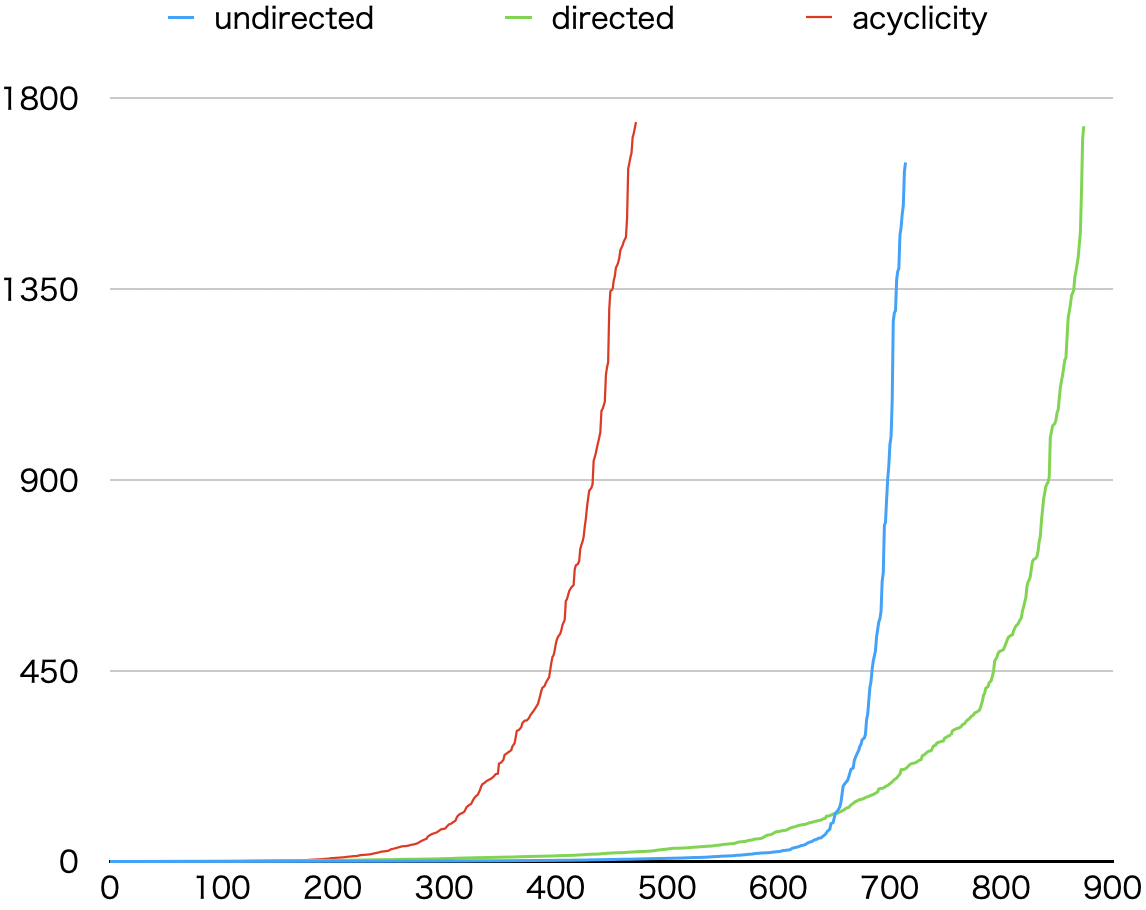
\includegraphics[width=0.8\linewidth]{fig/cactus_fhcp.png}
\caption{ハミルトン閉路問題: カクタスプロット}
\label{cactus}
\end{center}
\end{figure}
%%%%%%%%%%%%%%%%%%%%%%%%%%%%%%%%%%%%%%%%%%%%%%%


%--
本節では,ハミルトン閉路問題の実験結果について述べる.
{\clingo}のオプションは\textit{trendy}を使用し,一問あたりの時間制限を30分とした.
ベンチマーク問題は,\textsf{fhcp}の1001問である.

%--
表~\ref{sat_table}に,各符号化で解けた問題数を,問題の頂点数毎に示す.
左から,問題の頂点数,問題数,各符号化で解けた問題数を示している.
%
解けた問題数は,
\textsf{undirected}符号化が715問,
\textsf{directed}符号化が875問,
\textsf{acyclicity}符号化が473問であり,
\textsf{directed}がもっとも多くの問題を解いた.
\textsf{directed}は,どの頂点数においても同様に,
安定した性能の良さを示した.
図~\ref{cactus}に,カクタスプロットを示す.
縦軸は問題を解くのに要した CPU 時間,横軸は解けた問題数を表す.
グラフが右によるほど多くの問題を解けたことを示し,
下によるほどより速く解けたことを示す.
図~\ref{cactus}より,\textsf{directed}符号化が,
他の2つの符号化と比較して,より多くの問題を高速に解いていることが確認できた.
%% しかし,一部\textsf{undirected}符号化が\textsf{directed}符号化を下回る
%% 部分が確認できる.
%% 実際に,一部の問題では\textsf{undirected}符号化が
%% \textsf{directed}符号化よりも高速に解いていた.

%%%%%%%%%%%%%%%%%%%%%%%%%%%%%%%%%%%%%%%%%%%%%%%%%%%%%%%%%%
\subsection{最短ハミルトン閉路問題}
%%%%%%%%%%%%%%%%%%%%%%%%%%%%%%%%%%%%%%%%%%%%%%%%%%%%%%%%%%

%%%%%%%%%%%%%%%%%%%%%%%%%%%%%%%%%%%%%%%%%%%%%%%
\begin{table}[htbp]
  \caption{実験結果2-1:trendy}
  \label{min_table_tr}
  \centering
  \begin{tabular}{|l|rrr|}
    \hline
    Instance&undirected&directed&acyclicity \\
    \hline
    grid5&50,656*&50,656*&50,656* \\
    grid6&68,656*&68,656*&68,656* \\
    grid7&91,822*&91,822*&91,822* \\
grid8&113,250&\textcolor{red}{112,916}&113,277 \\
grid9&\textcolor{red}{142,502}&143,326&143,660 \\
grid10rc&\textcolor{red}{172,703}&174,866&175,999 \\
grid11&\textcolor{red}{200,399}&204,456&200,638 \\
grid12&\textcolor{red}{231,278}&239,275&232,012 \\
grid13&\textcolor{red}{276,692}&276,926&276,899 \\
grid14&317,617&\textcolor{red}{317,144}&317,676 \\
grid15&\textcolor{red}{375,906}&376,809&376,210 \\
grid16&421,249&\textcolor{red}{419,737}&423,753 \\
US48&11,698*&11,698*&11,698* \\
    \hline
  \end{tabular}
\end{table}
%\label{min_table_tr}
%%%%%%%%%%%%%%%%%%%%%%%%%%%%%%%%%%%%%%%%%%%%%%%

%--
本節では,最短ハミルトン閉路問題の実験結果について述べる.
{\clingo}のオプションは\textit{trendy}を使用し,
一問あたりの時間制限を3時間とした.
ベンチマーク問題は,\textsf{grid}と\textsf{usmap}の合計13問である.

%--
表\ref{min_table_tr}に,各符号化で得られた最適値と最良値を示す.
各問題毎に,最も良かった値を赤字で示している.
*マークは,最適値を表している.
最適値と最良値の数は,
\textsf{undirected}符号化が10問,
\textsf{directed}符号化が7問,
\textsf{acyclicity}符号化が4問であり,
\textsf{undirected}符号化の優位性が確認できた.

%%%%%%%%%%%%%%%%%%%%%%%%%%%%%%%%%%%%%%%%%%%%%%%%%%%%%%%%%%
\subsection{コスト制約付きハミルトン路問題}
%%%%%%%%%%%%%%%%%%%%%%%%%%%%%%%%%%%%%%%%%%%%%%%%%%%%%%%%%%

%%%%%%%%%%%%%%%%%%%%%%%%%%%%%%%%%%%%%%%%%%%%%%%
\begin{table*}[tb]\footnotesize
  \tabcolsep = 2mm
  %\renewcommand{\arraystretch}{1.0}
  \vskip .5em
  \centering
  \begin{tabular}{lr|rrr}
    \hline
    閾値(倍率)    &	解の総数 & \textsf{undirected} & \textsf{directed} & \textsf{acyclicity} \\
    \hline
    11698(1.00)   &	1      &\textbf{2.979} & 7.531 & 4.586	\\
    11814(1.01)   &	8      &5.587  & 15.322	& \textbf{5.250}	\\
    11931(1.02)   &	28     &\textbf{3.243}& 18.600	& 3.578	\\
    12282(1.05)   &	388    &10.003&19.818	& \textbf{6.296}	\\
    12867(1.10)   &	16,180  &16.548& 28.555	& \textbf{9.764}\\
    14037(1.20)   &	939,209 &48.262       &40.717	& \textbf{26.837}\\
    15207(1.30)   &	4,525,541&88.172      &55.276	& \textbf{42.037}\\
    16377(1.40)   &	6,702,964&99.154       &47.647	& \textbf{40.640}	\\
    17547(1.50)   &	6,876,526&95.390       &45.265	& \textbf{38.411}	\\
    18716(1.60)   &	6,876,928&98.937       &49.138	& \textbf{40.748}	\\
    \hline
    平均CPU時間 &   & 46.8275 & 32.7869  & \textbf{21.8147}\\\hline
%    Best    &   & 2 & 0 & \textbf{8} \\ \hline
  \end{tabular}
  \vskip .5em
  \caption{コスト制約付きハミルトン路問題: 解の全列挙に要した CPU 時間}
  \label{cost_table}
\end{table*}
%\label{cost_table}
%%%%%%%%%%%%%%%%%%%%%%%%%%%%%%%%%%%%%%%%%%%%%%%

%--
本節では,第~\ref{chap:background}章でも説明した
コスト制約付きハミルトン路問題(全列挙)の実験結果について述べる.
{\clingo}のオプションは\textit{crafty}を使用し,
一問あたりの時間制限を3時間とした.
ベンチマーク問題は,D.~E~.Knuth の教科書
The Art of Computer Programming~\cite{Knuth:TAOCP:SAT}
に記載されているグラフを使用した(図~\ref{fig:USmap}参照).
このグラフは,米国本土48州の隣接関係を表しており,
頂点数は48,辺の数は105である.
この問題の最短距離は 11698 である(表~\ref{min_table_tr}参照).
今回の実験では,
コスト制約を最短距離のN倍以下
($N=1.00,1.01,1.02,1.05,1.1,1.2,1.3,1.4,1.5,1.6$)として,解の全列挙を
行った.

%--
表~\ref{cost_table}に,各符号化が解の全列挙に要した CPU 時間を示す.
表の1列目はコスト制約の閾値と最短距離からの倍率,2列目は解の総数を表している.
各閾値毎に,最も良かった値を赤字で示している.
表より,
\textsf{acyclicity}符号化が,他の符号化と比較して,より多くの問題を
高速に解いていることがわかる.また,平均CPU時間も最も短い.
%%%%%%%%%%%%%%%%%%%%%%%%%%%%%%%%%%%%%%%%%%%%%%%%%%%%%%%%%%

%%% Local Variables:
%%% mode: latex
%%% TeX-master: "paper"
%%% End:

%%%%%%%%%%%%%%%%%%%%%%%%%%%%%%%%%%%%%%%%%%%%%%%%%%%%%%%%%%% 
\chapter{インクリメンタルな手法の提案} \label{chap:inc}
%%%%%%%%%%%%%%%%%%%%%%%%%%%%%%%%%%%%%%%%%%%%%%%%%%%%%%%%%%

XXX

%%% Local Variables:
%%% mode: latex
%%% TeX-master: "paper"
%%% End:

\chapter{おわりに}\label{chap:conc}

本論文では,電気制約として電流制約のみを考慮した配電網問題および配電網
遷移問題に対して,解集合プログラミング(ASP)を用いた解法を提案した.
配電網(遷移)問題に対する ASP を用いた研究は,著者らの知る限り,本論文
がはじめてである.
提案解法の特長と本論文の貢献について,以下にまとめる.

\begin{description}
\item[表現力:]
  配電網問題を解くための ASP 符号化を考案した.
  ASP 言語の高い表現力を生かし,
  配電網問題の制約を簡潔に記述できることを確認した.
  特に,有向符号化は,無向グラフの各辺$u-v$に対して,2つの弧
  $u\rightarrow v$と$v\rightarrow u$を対応させることで有向グラフ化して
  解く符号化であり,非閉路制約を簡潔に表現できる点が特長である.
\item[拡張性:]
  配電網遷移問題に対して,マルチショット ASP 解法を利用した符号化を提案した.
  この符号化は,配電網問題の ASP 符号化の自然な拡張となっている.
  マルチショット ASP 解法を利用することにより,
  ASP システムが同様の探索失敗を避けるために獲得した学習節を
  (部分的に)保持することで,無駄な探索を避けることができる点が特長である.
\item[効率性:]
  DNET (Power Distribution Network Evaluation Tool)
  に公開されている配電網問題(全3問)と,
  Graph Coloring and its Generalizations
  に公開されているグラフを基に独自に生成したトポロジ制約のみの配電網問
  題(計82問)を用いて実行実験を行なった.
  その結果,有向符号化は,他の2つの符号化と比較して,より多くの問題を
  より高速に解くことができ,その優位性を確認できた.
  %
  配電網遷移問題については,実用規模の問題({\sf fukui-tepco})に対して,
  実行可能解のペアをランダムに選び,合計 1000 問の配電網遷移問題を生成
  し,実行実験を行なった.その結果,すべての問題の到達可能性を判定する
  ことができ,得られた最短ステップ長の最大値は7であった.また,
  マルチショットASP解法を導入することにより,
  通常の解法と比較して,平均で3.8倍の高速化を実現した.
\end{description}

今後の課題としては,電流制約と電圧制約を含む完全な配電網問題への拡張が
挙げられる.しかし,完全な問題は非線形な制約を含むため,標準的な ASP
言語では記述できない.この問題を解決するために,近年研究開発が進められ
ている背景理論付き ASP (ASP Modulo Theories~\cite{DBLP:conf/iclp/GebserKKOSW16}) 
を用いた解法の実現可能性について調査を進める.

%%% Local Variables:
%%% mode: japanese-latex
%%% TeX-master: "paper"
%%% End:

% ここまで

%%%%%%%%%%%%%%%%%%%%%%%%%%%%%%%%%%%%%%%%%%%%%%%%%%%%%%%%%% 
\chapter*{謝辞}
%%%%%%%%%%%%%%%%%%%%%%%%%%%%%%%%%%%%%%%%%%%%%%%%%%%%%%%%%%

本研究を行うにあたり,
研究の着想から論文執筆にわたり
熱心なご指導を頂いた名古屋大学の番原 睦則教授
に深く感謝申し上げます.
また,本研究だけではなく,様々な相談に乗っていただいた
番原研究室の皆様に感謝申し上げます.
最後に,大学生活を通して支えていただいた家族,友人に
感謝申し上げます.


%%% Local Variables:
%%% mode: japanese-latex
%%% TeX-master: "paper"
%%% End:         % 謝辞

\bibliographystyle{jplain} % 参考文献スタイル
\bibliography{bachelor,aisat}    % 参考文献リスト

\end{document}
%%%%%%%%%%%%%%%%%%%%%%%%%%%%%%%%%%%%%%%%%%%%%%%%%%%%%%%%%%

%%% Local Variables:
%%% mode: japanese-latex
%%% TeX-master: t
%%% End:
